\documentclass[12pt]{iopart}
\pdfminorversion=4
%Uncomment next line if AMS fonts required
%\usepackage{iopams}
\usepackage{myphysics} %units, particles and misc definitions from ATLAS
\usepackage{graphicx}  %\includegraphics...
\usepackage{subfigure}

\begin{document}

\title[Electroweak phyiscs at the LHC]{Electroweak physics at the LHC}
\author{J Berryhill$^1$ and A Oh$^2$}

\address{$^1$ Fermi National Accelerator Laboratory, Batavia, IL, USA}
\address{$^2$ School of Physics and Astronomy, University of Manchester, Manchester, UK}

%\ead{submissions@iop.org}
%\vspace{10pt}
%\begin{indented}
%\item[]February 2014
%\end{indented}

\begin{abstract}
The Large Hadron Collider (LHC) has completed in 2012 its first
running phase and the experiments have collected data sets of proton-proton
collisions at center-of-mass energies of 7 and 8 \TeV\xspace with an
integrated luminosity of about 5 and 20 \ifb, respectively.  Analyses
of these data sets have produced a rich set of results in the
electroweak sector of the standard model. This article reviews the
status of electroweak measurements of the ATLAS and CMS experiments at
the LHC.
\end{abstract}

% Uncomment for PACS numbers
\pacs{12.15.-y, 12.60.Cn, 14.70.-e}
%
% Uncomment for keywords
%\vspace{2pc}
%\noindent{\it Keywords}: XXX, YYY, ZZZ
%
% Uncomment for Submitted to journal title message
\submitto{\jpg}
%
% Uncomment if a separate title page is required
\maketitle
%
% For two-column output uncomment the next line and choose [10pt] rather than [12pt] in the \documentclass declaration
%\ioptwocol
%


\section{Introduction}
%\subsection{Motivation to study the electroweak sector}
\label{ss-intro-motivation}

%Physics motivation
With the discovery of the Higgs boson in 2012~\cite{Chatrchyan201230, Aad20121} 
the standard model of particle physics
seemed complete, but fundamental questions remaine to be answered, as for example about the
constituents of dark matter, the relative abundance of matter over anti-matter, 
and the unification of forces at the Planck scale. 

%EWK precision measurements
Precision measurements in the electro-weak sector allow to test the validity of 
various extensions of the standard model. In the framework of anomalous gauge couplings
and it's reformulation as effective field theory the standard model can be extended
with additional generic terms in the lagrangian to describe new physics. The 
measurement of electroweak production processes allows to verify the validity 
of the standard model in this framework at the high collision energies the LHC
is providing.

% photon structure and benchmark perturbative QCD
Beside eletroweak measurements, the proton-proton collisions at the LHC provide a rich testing ground to 
benchmark perturbative QCD over a wide range of scales, and to determine the structure
of the proton. Both are essential ingredients to make precise eletroweak measurements, as higher order
corrections in perturbative QCD have a substantial effect on the theoretical predictions to 
standard model processes, and the knowledge of the proton structure becomes a major uncertainty
for processes with very high partonic centre of mass, i.e. the region where we expect new physics
to become visible.

%LHC and detectors
The Large Hadron Collider (LHC) was designed to search for the Higgs boson and
new phenomena. 

%LHC machine
The LHC collides protons on protons in a circular ring of 27\;km 
circumference and can reach an energy of up to $7\TeV$ per beam, and a collision
energy at the centre-of-mass of up to $\rts=14\TeV$. 

%Detectors
The two general purpose detectors at the LHC, ATLAS and CMS, are able to
record a wide range of physics process. They differ in the technical details of detector
layout and data-acquisition design but have common design goals, namely 
good detector coverage for charged and neutral particles, excellent resolution to measure
the positions and momenta of charged particles, and precision calorimetry. The other two
main experiments at the LHC are optimized for recording collision of heavy ions in the 
case of ALICE or for precision measurements of b-hadrons and CP violation (LHC-b).

% electroweak objects produced in run-1
% W,Z produced, di-boson final states? 
% MW mass, prospects vs reality?

% mention typical systematic uncertainties on leptons, jets, met

% mention ewk parameters from LHC in PDG?




%outline
In the following we will briefly review the electroweak physics programme at the LHC (section~\ref{ss-lhc-physics}),
followed by an overview of theory developments (section~\ref{s-theory-overview}), and a comprehensive
summary of the electroweak results from ATLAS and CMS on inclusive vector boson production in section~\ref{s-inclusboson} 
and electroweak precision tests in section~\ref{s-ewk-prec-tests}. 


%\subsection{Electroweak physics at hadron colliders}
%\subsection{LHC physics program}
%\input{ss-lhc-physics}
%\subsection{Electroweak challenges for Run 2 and beyond}
\section{Theory overview and recent developments}
\label{s-theory-overview}

We confine discusion of results in this review to experimental tests
at the LHC which directly and uniquely test the electroweak
interactions of the known standard model particles, excluding the
Higgs boson. A simple but general framework to study those
interactions is through effective field theory extensions of the
standard model which respect the standard model $SU_C(3) \otimes
SU_L(2) \otimes U_{EM}(1)$
symmetry~\cite{Weinberg:1978kz,Weinberg:1980wa,Georgi:1994qn}.  These
extensions can be generally written in an operator product expansion
(OPE)

$$ \mathcal{L} = \mathcal{L}_{SM} + \sum_i \frac{c_i}{\Lambda^{2n}}{\cal O}_i + \cdots$$

where $c_i$ are dimensionless coefficients, $\Lambda$ is some energy
scale corresponding to the scale of new physics, and ${\cal O}_i$ are
operators constructed from Standard Model fields.  In principle, given
an ultraviolet-complete theory of new physics with possibly new
particle content, the $c_i$ at the electroweak scale are calculable
and can be compared with the observed experimental footprint. In the
context of electroweak studies, especially for the study of
gauge-boson self-interactions, this is often restricted to $CP$-even
operators of mass dimension six (the
lowest allowable).  In that case, there are only three independent
operators with three independently measurable Wilson coefficients. The
precise definition of the independent coefficents depends upon the
basis chosen to express the operators.  The most common contemporary
convention is the LEP basis, for which the coefficients are labeled
$c_{WWW}$, $c_W$, and $c_B$~\cite{Hagiwara:1993ck,Degrande:2012wf},
which correspond to combinations of $WW\gamma$ and $WWZ$ interactions.
Prior to the most recent Run 1 results, these same operators (up to a
simple linear combination) were constrained via dimensionless
couplings, known as $\lambda$, $\kappa$, and $g_1$; these can be
easily translated into the Wilson coefficients $c_i$ by a linear
transformation~\cite{Degrande:2012wf}.  By measuring total or
differential cross sections of processes which isolate triple gauge
boson self-interactions (TGCs), predictions from the EFT can be
compared to the data and allow for bounding the values of the
coefficents, typically expressed as the dimensionful ratio
$c_i/\Lambda^2$.

In understanding all of the conceivable quartic gauge boson
interactions (QGCs), it is useful to also consider EFTs for which
dimension 6 operators are suppressed, and the leading order OPE has
terms of mass dimension 8, with dimensionful coefficients
$c_i/\Lambda^4$.  Dimension 8 theories have up to 19 independent gauge
boson self-interaction operators, including the following quartic
combinations: $WWWW$, $WWZZ$, $WWZ\gamma$, $WW\gamma\gamma$, as well
as non-SM interactions $ZZZZ$, $ZZZ\gamma$, $ZZ\gamma\gamma$, and
$Z\gamma\gamma\gamma$~\cite{Eboli:2006wa,Degrande:2013kka}.

Not all $c_i/\Lambda^n$ give rise to unitary or perturbatively
calculable field thoeries, therefore care must be taken to specify,
for each experimental observable, which range is applicable.
Alternatively, some (higher mass dimension) unitarization procedure
can be adopted: an energy cutoff on the cross section, a form factor
which moderates the high-energy behavior (usually of the form
$(1+q^2/\Lambda^2)^{-2}$), or a $K$-matrix unitarization
procedure~\cite{Alboteanu:2008my,Chung:1995dx}.  In general, the Run 1
data on dimension-6 EFTs do not explore the range of coefficients and
energies which would escape unitarity bounds, in which case the bare
results have a straightforward interpretation.  It is typical,
however, for dimension-8 EFTs to spoil unitarity in the Run 1 LHC
energies and sensitivities, so the details of unitarity and
unitarization are critical in presenting and interpreting those
results.

Another framework for testing the electroweak theory is through global
fits of the SM electroweak parameters to the high-precision
electroweak data available in $W$ and $Z$ production.  Poor
goodness-of-fit for one or more precision observables is indicative of
new electroweak interactions at the loop level contributing to
electroweak boson production and decay; these constraints can also be
translated into bounds on EFT coefficients.  The most recent global
fits~\cite{Baak:2014ora,Ciuchini:2013pca} include, among others, the
LEP and SLD precision data in $Z$ production, the Tevatron measurement
of the $W$ mass, and the high-precision measurements of the top quark
and Higgs boson masses at the LHC.  These fits generally predict
values for the $W$ mass and weak-mixing angle $\sin^2\theta^{eff}_{W}$
more accurate than have been directly obtained, providing an
opportunity at the LHC to over-constrain the global fit further.

Improving upon either of these frameworks for electroweak model
parameters at the LHC is only possible with state-of-the-art
understanding of perturbative QCD, parton distribution functions
(PDF), and electroweak radiative corrections.  In general, for Run 1
LHC results multiboson production has been studied with
next-to-leading order (NLO) QCD matrix elements combined with parton
showering to provide a particle-level simulation and some emulation of
higher-order radiative and non-perturbative corrections. The PDFs and
underlying event modelling typically include the LHC data themselves.
For precision single boson production next-to-next-to-leading order
(NNLO) calculations were used, along with NLO electroweak radiative
corrections.  The LHC data typically improve upon contemporary PDFs in
this domain, motivating precision measurement of boson production to
constrain them further.  In the future, multiboson and vector-boson
scattering studies will require NNLO QCD and NLO electroweak matrix
elements, parton-shower matching at that order, and PDFs consistently
provided at that order including all of the Run 1 LHC data, as the Run
1 data are already precise enough to be sensitive to these effects in
some areas.


\section{Inclusive boson production}
\label{s-inclboson}

\subsection{Drell-Yan production}
\label{ss-inclboson-drellyan}
At a hadron collider, the most fundamental tests of electroweak boson
couplings to fermions are measurements of the kinematic properties of
Drell-Yan (DY) lepton pair production.  At leading order, Drell-Yan
production occurs when a quark--anti-quark pair in the intial state
annihilates into an electroweak boson, which subsequently decays to a
lepton pair. Differential cross section calculations exist for
next-to-next-to leading order (NNLO) QCD corrections as well as NLO
electroweak corrections. In the EFT context, such a process is
sensitive to four-fermion contact interactions of the type

\begin{equation}\label{lagrangian}
\begin{array}{r@{\,}c@{}c@{\,}l@{\,}l}
\mathcal L = \frac{g^2}{\Lambda^2}\;[ && \eta_{\rm LL}&\, (\overline q_{\rm L}\gamma_{\mu} q_{\rm L})\,(\overline\ell_{\rm L}\gamma^{\mu}\ell_{\rm L}) \nonumber \\
& +&\eta_{\rm RR}& (\overline q_{\rm R}\gamma_{\mu} q_{\rm R}) \,(\overline\ell_{\rm R}\gamma^{\mu}\ell_{\rm R}) \\
&+&\eta_{\rm LR}& (\overline q_{\rm L}\gamma_{\mu} q_{\rm L}) \,(\overline\ell_{\rm R}\gamma^{\mu}\ell_{\rm R}) \\
&+&\eta_{\rm RL}& (\overline q_{\rm R}\gamma_{\mu} q_{\rm R}) \,(\overline\ell_{\rm L}\gamma^{\mu}\ell_{\rm L})& ] \: ,\nonumber
\end{array}
\end{equation}
where $g$ is a coupling constant, $\Lambda$ is the contact interaction scale,
and $q_{\rm L,R}$ and $\ell_{\rm L,R}$ are left-handed and right-handed quark and
lepton fields, respectively. The parameters $\eta_{i,j}$ denote the relative interference of the operators;
the experiments have considered the cases $\eta_{\rm LR} = \eta_{\rm RL} = \pm 1$,
$\eta_{\rm LL} = \pm 1$, or $\eta_{\rm RR} = \pm 1$.

Experiments select electron or muon pairs above trigger thresholds:
CMS selects leading lepton $\pt >$ 17 GeV and second leading lepton
$\pt >$ 8 GeV inclusively, and ATLAS selects high mass events with
both lepton $\pt >$ 25 GeV.  Backgrounds to Drell-Yan production are
relatively small, and consist of real prompt lepton pair production
from top quark or boson pairs, as well as fake electrons from QCD
jets.  The real lepton pair background is flavor democratic, and can
therefore be reliably estimated from $e\mu$ pair production.  Fake
electron production is typically estimated from background enriched
QCD jet samples, from which the fake electron rate can be measured,
convolved with electron-jet control samples.

Figure~\ref{fig:ss-inclboson-drellyan-atlas7tev} shows the Drell-Yan
cross section at high electron pair mass measured by ATLAS at 7
TeV~\cite{Aad:2013iua}.  The cross section uncertainty is
predominantly systematic below 400 GeV in pair mass and predominantly
statistical above 400 GeV.  The data are compared with an NNLO QCD
prediction with NLO electroweak corrections, provided by the
\texttt{FEWZ} 3.1
generator~\cite{Melnikov:2006kv,Gavin:2010az,Li:2012wna}.  The
prediction also includes photon induced lepton pair production, which
generally increases cross section estimates by a few percent. The
\texttt{FEWZ} prediction generally underestimates the cross section,
however a correlated chi-squared analysis concludes that this is not
statistically significant.

Figure~\ref{fig:ss-inclboson-drellyan-cms8tev} shows the Drell-Yan
cross section for electron or muon pairs measured by CMS at 8
TeV~\cite{CMS:2014jea}.  Agreement with the \texttt{FEWZ} prediction
is observed over the entire measured mass range, from 15 GeV to 2000
GeV.  CMS has also measured the double differential cross section with
respect to dilepton rapidity in several bins of dilepton mass, as well
as a differential cross section ratio between the 8 TeV and 7 TeV
data, which has small experimental and theoretical uncertainties.

In the absence of observed disagreements with predictions at the
highest dilepton masses, the data are analyzed to constrain the size
of anomalous contact interactions. Assuming a fixed, strong value for
the coupling ($g^2/4\pi = 1$), limits can be obtained on the contact
interaction scale $\Lambda$.  ATLAS estimates a lower limit of 17 to
26 TeV on $\Lambda$, where the strongest lower limits correspond to
constructive interference scenarios (especially LR+RL), and the
weakest to destructive interference scenarios~\cite{Aad:2014wca}.  CMS
has limits with similar sensitivity estimated for LL contact
interactions~\cite{Khachatryan:2014fba}.

%ATLAS low-mass Drell-Yan $7 \TeV$~\cite{Aad:2014qja}
%ATLAS Z PT $7 \TeV$~\cite{Aad:2014xaa}
%ATLAS Z phistar $7 \TeV$~\cite{Aad:2012wfa}
%CMS Drell--Yan $7 \TeV$~\cite{Chatrchyan:2013tia}
%CMS angular coefficients $8 \TeV$~\cite{Khachatryan:2015paa}
%CMS Z PT and rapidity $8 \TeV$~\cite{Khachatryan:2015oaa}
%CMS dilepton contact interactions~\cite{Khachatryan:2014fba}
%ATLAS dilepton contact interactions~\cite{Aad:2014wca}

\begin{figure}[p]
    \centering
    \includegraphics[height=0.3\textheight]{figures/ss-inclboson-drellyan-atlas7tev}
    \caption{Measured differential cross-section at the Born level within the
    fiducial region (electron $\pt > 25 \GeV$ and $|\eta| < 2.5$) with statistical,
     systematic, and combined statistical and systematic (total) uncertainties,
     excluding the 1.8\% uncertainty on the luminosity.
      On the left, in the upper ratio plot, the photon-induced (PI)
     corrections have been added to the predictions obtained from the MSTW2008,
     HERAPDF1.5, CT10, ABM11 and NNPDF2.3 NNLO PDFs, and for the MSTW2008 prediction
     the total uncertainty band arising from the PDF, $\alpha_s$, renormalisation
     and factorisation scale, and photon-induced uncertainties is drawn. The lower
     ratio plot shows the influence of the photon-induced corrections on the
     MSTW2008 prediction, the uncertainty band including only the PDF, $\alpha_s$
     and scale uncertainties.}
    \label{fig:ss-inclboson-drellyan-atlas7tev}
\end{figure}

\begin{figure}[p]
    \centering
    \includegraphics[height=0.3\textheight]{figures/ss-inclboson-drellyan-cms8tev}
    \caption{The DY differential cross section as measured in the combined
dilepton channel and as predicted by NNLO \texttt{FEWZ} 3.1 with CT10 PDF
calculations, for the full phase space.}
    \label{fig:ss-inclboson-drellyan-cms8tev}
\end{figure}


\subsection{Inclusive di-boson production}
%short intro
The production of \ZZ in proton-proton collisions has been one of the first di-boson 
processes measured at the LHC. The SM process is and an important and irreducible
background to resonance searches and Higgs production. The production at leading
order is dominated by quark anti-quark annihilation in the $t$ and $u$-channel,
whereas the $s$-channel process is forbidden in the SM 
(see also Figure~\ref{fig:sss-ZZprod-LOdiagrams}). The gluon fusion process 
contributes about 6\% to the total production cross section. 

%FIGURE LO ZZ DIAGRAM
\begin{figure}[htbp]
  \begin{center}
  \includegraphics[width=0.9\textwidth]{figures/sss-inclboson-diboson-zzprod-zzdiagram.png}
  \caption{Leading order Feynman diagrams of \ZZ production in the dominant 
  \qqbar\ channel. The \ZZ\ production via the $s$-channel is not allowed in the SM.}
\label{fig:sss-ZZprod-LOdiagrams}
\end{center}
\end{figure}

%decay channels
Precision measurements use the leptonic decay modes of the $Z$ to reduce the impact of
QCD backgrounds. 
The four lepton final state provides an almost background free signature, at the
expense of a relatively small branching ratio 
$BR(ZZ) \to \ll\ll = 0.101^2 \cdot {4 \over 9} = 0.0045$~\cite{PDG}.  
The di-lepton and missing energy channel can exploit the one order of magnitude
higher branching ratio of 
$BR(\ZZ \to \ll\vv) = 0.101 \cdot 0.20 \cdot 2 \cdot {2 \over 3} = 0.0269$, 

%analysis CMS and ATLAS.
%ATLAS ZZ 7 TeV~\cite{Aad:2012awa}
%CMS ZZ4l 8 TeV~\cite{Khachatryan:2014dia}
%CMS ZZ4l 7 TeV~\cite{Chatrchyan:2012sga}
%CMS ZZ2l2nu 7+8 TeV~\cite{Khachatryan:2015pba}
The ATLAS collaboration has published results on the $7\TeV$ data-set 
in the $\ll\ll$ and $\ll\vv$ final state~\cite{Aad:2012awa}. The CMS collaboration
has analysed the full 7 and $8\TeV$ data sets in both 
the $\ll\ll$~\cite{Chatrchyan:2012sga,Khachatryan:2014dia} and 
$\ll\vv$ final state~\cite{Khachatryan:2015pba}.

%Theoretical calculations
% NLO alpha_s arXiv:1105.0020
% NLO alpha_EKW arXiv:1305.5402,arXiv:1307.4331
Theoretical predictions for $\ZZ$ production are available 
at NLO in $\alpha_s$~\cite{arXiv:1105.0020}. In addition, electroweak 
corrections at NLO have been calculated~\cite{arXiv:1305.5402,arXiv:1307.4331}. 

%Selections
The event selection for the $\ll\ll$ final state requires exactly four leptons 
fulfilling a set of cuts on kinematic quantities. ATLAS and CMS use similar criteria 
as listed in detail in Table~\ref{tab:sss-ZZprod-cuts}. While ATLAS uses $l=e,\mu$,
CMS includes also $\Z\to\tautau$ with subsequent hadronic and leptonic $\tau$
decays. ATLAS uses in addition forward leptons outside the ID tracker
to increase the acceptance by 6\% for electrons and 10\% for muons.

%Backgrounds

% Results at the end?
Besides the total cross section for the $pp \to \ZZ$ production process, both
experiments measure also fiducial and differential cross sections, and provide
limits on anomalous neutral triple gauge boson couplings.






\subsubsection{WZ production}

\label{sss-WZprod}

%short intro
At the LHC, \WZ\ di-bosons are produced from quark-antiquark initial states at 
leading order and quark-gluon initial states at next-to-leading order. %~\cite{PhysRevD.65.094041}
%Figure~\ref{fig:LOdiagrams} shows the LO Feynman diagrams for \WZ production from $q\bar{q}'$ initial states. 
The SM-allowed $s$-channel diagram has a triple boson vertex and is sensitive to 
ATGC.

%FIGURE LO WZ DIAGRAM
% may include 
% figures/sss-inclboson-diboson-wzprod-wz-s-channel.pdf
% figures/sss-inclboson-diboson-wzprod-wz-t-channel.pdf
% figures/sss-inclboson-diboson-wzprod-wz-u-channel.pdf

%\begin{figure}[htbp]
%  \begin{center}
%  \includegraphics[width=0.9\textwidth]{figures/sss-inclboson-diboson-wzprod-wzdiagram.png}
%  \caption{Leading order Feynman diagrams of \WZ production in the dominant 
%  \qqbar\ channel.}
%\label{fig:sss-WZprod-LOdiagrams}
%\end{center}
%\end{figure}

%decay channels


%analysis CMS and ATLAS.
%ATLAS WZ 8 TEV \cite{Aad:2016ett} 
%ATLAS WZ 7 \TeV~\cite{Aad:2012twa}
% - figure from https://atlas.web.cern.ch/Atlas/GROUPS/PHYSICS/PAPERS/STDM-2012-09/
%CMS WZ at 7+8 \TeV (CMS-PAS-SMP-12-006, to be published)
The ATLAS experiment measured the \WZ\ production cross section in the fully 
leptonic decay channel \ll\lnu\; at $\rts = 7\TeV$~\cite{Aad:2012twa} and $\rts = 8\TeV$~\cite{Aad:2016ett} 
and set limits on charged ATGC.
%Theoretical calculations
% TBD
% WZ->lllv
%Selections
In these analyses the final states involving electrons or muons are considered as signal,
whereas boson decays to taus are considered as background.  
%Backgrounds
The dominant background sources are \Zboson+jet and \ZZ production, accounting for about 40\% of 
the overall background. The overall signal to background ratio is about $4$.
%systematics
The leading systematic uncertainty is related to the data-driven estimation method of the   
background.%, with the dominant Z + jets contributing ($\pm3.8\%$).

% Results at the end
% xsec
The fiducial cross section for the 7 TeV (8 TeV) analysis is defined by $\pt^{\mu,e} > 15\GeV$ for the leptons from the \Zboson\ 
 decay, $\pt^{\mu,e} > 20\GeV$ for the lepton from the \Wboson, $|\eta^{\mu,e}|<2.5$, $\pt^\nu>25\GeV$,
 $|m_ll-m_Z| < 10(25)\GeV$, $M_T^W>20(30)GeV$ and $\Delta R> 0.3$ for the three possible $\ell\ell$ pairings. 
The total cross section requires the mass of the \Zboson\ to be in the range of $66\GeV < |m_Z| < 116\GeV$
to suppress the contribution from $\gamma^*$.
The fiducial and total cross sections are compared to the SM expectation at NLO in Table~\ref{tab:sss-WZprod-xsec}.

\begin{table}[htp]
\begin{center}
\resizebox{\textwidth}{!}{
\begin{tabular}{|c|c|c|c|c|c|}
Experiment & cross section & \rts\;[TeV] & measured  & predicted  & reference  \\ \hline
ATLAS & total & 7  & {19$^{+1.4}_{-1.3}$ (stat.) $\pm{0.9}$ (syst.) $\pm$ 0.4 (lumi.) pb}  & {17.6 $^{+1.1}_{-1.0}$ pb} & \cite{Aad:2012twa} \\
ATLAS & total & 8  & {24.3$\pm 0.6$ (stat.) $\pm{0.6}$ (syst.) $\pm{0.4}$ (theo.) $\pm$ 0.5 (lumi.) pb}  & {21.0  $\pm$ 1.6 pb} & \cite{Aad:2016ett} \\
ATLAS & fiducial & 7  & {92 $^{+7}_{-6}$ (stat.) $\pm{4}$ (syst.) $\pm$ 2 (lumi.) fb}  & -- & \cite{Aad:2012twa} \\
ATLAS & fiducial & 8  & {35 $\pm{0.9}$ (stat.) $\pm{0.8}$ (syst.) $\pm$ 0.8 (lumi.) fb}  & {30$\pm{0.5}$ (PDF) $\pm{0.8}$ (scale) fb} & \cite{Aad:2016ett} \\
\end{tabular}
}
\caption{Summary of measured fiducial and total $\WZ$ production cross sections from ATLAS 
at 7 TeV center-of-mass energies in the $\ll\lnu$ final state. The fiducial definitions differ from the 7 and 8 TeV analysis. Furthermore, the 7 TeV analysis
quotes the sum for the $e$ and $\mu$ channels, the 8 TeV analysis quotes the combination of channels. Thus, the two fiducial cross sections cannot be 
compared directly.}
\end{center}
\label{tab:sss-WZprod-xsec}
\end{table}%


% unfolded spectra
In Figure~\ref{fig:sss-WZprod-ptZ-det} the differential cross section measured in bins of 
$\pt^Z$ is shown, compared to SM prediction and a set of anomalous TGC couplings. 
The normalized $\pt^Z$ spectrum is unfolded and compared to the NLO calculation of \mcatnlo in 
Figure~\ref{fig:sss-WZprod-ptZ-det}, showing good agreement with the SM.


\begin{figure}[htbp]
  \begin{center}
  \includegraphics[width=0.45\textwidth]{figures/sss-inclboson-diboson-wzprod-ptZ-det.pdf}
  \caption{ATLAS measurement of the transverse momentum of the \Zboson in \WZ events ($\pt^Z$) compared with the SM prediction at $\rts = 7\TeV$. For illustration, calculations for a set of anomalous couplings values are also shown. The full uncertainty contains statistical and systematic uncertainties.}
\label{fig:sss-WZprod-ptZ}
\end{center}
\end{figure}

\begin{figure}[htbp]
  \begin{center}
  \includegraphics[width=0.45\textwidth]{figures/sss-inclboson-diboson-wzprod-ptZ.pdf}
  \caption{ATLAS measurement of the normalized fiducial cross-sections in bins of $\pt^Z$ compared with the SM prediction at $\rts = 7\TeV$. The full uncertainty contains statistical and systematic uncertainties.}
\label{fig:sss-WZprod-ptZ-det}
\end{center}
\end{figure}


%%%%
% THIS MIGHT GO INTO THE SECTION ON TGC
% aTGC
Limits on the charged ATGC parameters \dkz, \lz\ and \gz\ are extracted from the transverse momentum distribution
of the \Zboson, $\pt^Z$~\cite{Aad:2012twa} or from the transverse mass of the $\Wboson\Zboson$ system~\cite{Aad:2016ett}. 
The ATGC parameter 95\% CL limits using a dipole form factor with a cut-off of $\Lambda=2\TeV$ and without a form factor are quoted 
in Table~\ref{tab:sss-WZprod-ATGC} from the more constraining $8\TeV$ data set analysis~\cite{Aad:2016ett}.

%\begin{table}\centering
%\caption{Expected and observed 95\% CL on 
%\dkz, \lz\ and \gz.}
%\label{tab:sss-WZprod-ATGC}
%\begin{tabular}{ccccc}
%\hline
%& $\rts$,  & Observed & Observed & Expected \\
%& & $\Lambda=2$~TeV & no form factor & no form factor\\
%\hline
%$7\TeV$ & $\gz$ & $[-0.074, 0.133]$ & $[-0.057, 0.093]$ & $[-0.046, 0.080]$ \\
%$7\TeV$ & $\dkz$ & $[-0.42, 0.69]$ & $[-0.37, 0.57]$ & $[-0.33, 0.47]$ \\
%$7\TeV$ & $\lz$ & $[-0.064, 0.066]$ & $[-0.046, 0.047]$ & $[-0.041, 0.040]$ \\
%\hline
%\end{tabular}
%\end{table}


\begin{table}\centering 
\begin{tabular}{cccc}
\hline
 $\Lambda$ & Coupling & Expected  & Observed \\
\hline
2 TeV 	& $\gz$ 		& [$-0.023$, $0.055$]  & [ $-0.029$, $0.050$] \\
2 TeV 	& $\dkz$ 	& [$-0.17$, $0.25$]    & [$-0.19$, $0.30$] \\
2 TeV 	& $\lz$ 	& [$-0.016$, $0.016$]  & [$-0.016$, $0.016$] \\
\hline
\end{tabular}
\caption{Expected and observed 95\% CL on \dkz, \lz\ and \gz\; for a cut-off parameter $\Lambda = 2\TeV$ and $\Lambda = \infty$.}
 \label{tab:sss-WZprod-ATGC}
\end{table}
 

% WZ->llqq ????











\subsubsection{WW production}
\label{sss-WWprod}

%short intro
The \WW\ production process has the highest production cross section
among the massive vector diboson processes. It is also an important
background process to Higgs production and to searches for new physics.
%analysis CMS and ATLAS.
%    ** ATLAS (5.6ifb, 7TeV, TGC), Phys. Rev. D 87, 112001 (2013), http://arxiv.org/abs/1210.2979
%	    ATLAS (20ifb 8TeV), https://atlas.web.cern.ch/Atlas/GROUPS/PHYSICS/CONFNOTES/ATLAS-CONF-2014-033/ 
%    ** CMS (7 TeV, 5 fb-1, TGC)  WW cross section in the lvlv channel at 7 TeV  http://arxiv.org/abs/1306.1126
%    ** CMS (8 TeV, 3.5 fb-1 WW, 5.3 fb-1 ZZ) , Phys. Lett. B 721 (2013) 190, WW and ZZ at 8 TeV, http://arxiv.org/abs/1301.4698 
%	    CMS (20ifb, 8TeV), submitted to EPJC,  http://arxiv.org/abs/1507.03268
ATLAS and CMS, observed the \WW\ production process in 
the fully leptonic channel and published results for 7 TeV 
(ATLAS~\cite{ATLAS:2012mec},CMS~\cite{Chatrchyan:2013yaa}) and
8 TeV (CMS~\cite{Chatrchyan:2013oev}) centre-of-mass energy. 
%decay channels
Three final states, namely $ee$, $\mu\mu$, and $e\mu$ are included in the analyses. 
The contribution from leptonically decaying $\tau$ leptons is included in the signal
definition. Although the production cross section is relatively high, the signature of two opposite 
sign leptons and missing transverse energy is shared with many processes and a careful
control of the backgrounds is necessary to achieve a precise measurement.

%Theoretical calculations
% TBD -> General section about theoretical calculations?

%Selections
Candidate $\WW$ events are selected by by requiring two oppositely charged leptons 
accompanied with large \MET. 
%Backgrounds
The dominant background sources are \ttbar\; and single top quark, 
$\W/$+jets, followed by $\Zzero/\gamma^{*}$+jets production.
To suppress the dominant \ttbar\; background, events with one or more jets are rejected.   
Additional requirements on \MET\ and the use of top quark-taggers further reduce the residual background
%ATLAS: 685 WW, 275 background => b / (s+b) = 29%
%CMS: 824WW, 369 background => b / (s+b) = 31%
to about 30\%.  
%systematics
The dominant systematic uncertainty is related to the jet veto efficiency 
and estimated to about 5\% for the \WW\, production. 
The experiments quote a theoretical uncertainties on the signal acceptance due to 
variations of the parton distribution functions and renormalisation and factorization 
scale in the range of 1-2\%.

% Results at the end
% total xsec
% ATLAS 7TeV 4.6 ifb: xsec(WW) = 51.9 +- 2.0 (stat) +- 3.9 (sys) +- 2.0 (lum) pb
%                     xsec_theo(WW) = 44.7 +2.1 -1.9 pb
% CMS 7TeV 4.9 ifb: xsec(ww) = 52.4 +- 2.0 (stat) +- 4.5 (syst) +- 1.2 (lum) pb
%                   xsec_theo(WW) = 47.0 +- 2.0 pb
% CMS 8TeV 5ifb: xsec(WW) = 69.9 +- 2.8 (stat) +- 5.6 (sys) +- 3.1 (lum) pb
%                xsec_theo(WW) = 57.3 +2.3 -1.6 pb (not including H ~ 4%)

% definition of total xsecs might differ (inclusion of higgs or not).
Both ATLAS and CMS provide a measurement of the total cross section for the process $pp \rightarrow \WW$
and compare to theoretical calculations. The Higgs process contributes with about 4\% to the total 
cross section and has not been taken into account in the comparison to the SM predictions.
The total cross section results are summarised in Table~\ref{tab:sss-WWprod-xsec}.
A good agreement of the experiments for the measured cross section as well as for the theoretical predictions
is observed.
% fiducial xsec
A normalised differential measurement of the fiducial cross section in bins of $\pt$ of the leading lepton is presented by ATLAS,
as shown in Figure~\ref{fig:sss-WWprod-pt-fiducial}. The unfolded spectrum is in agreement with the SM prediction.

\ref{tab:sss-WWprod-xsec}.
\begin{table}[htp]

\begin{center}
\resizebox{\textwidth}{!}{
\begin{tabular}{|c|c|c|c|c|c|}
Experiment & cross section & \rts & measured  & predicted  & reference  \\ \hline
ATLAS & total & 7 GeV & {51.9 $\pm 2.0$  (stat.) ${3.9}$ (syst.) $\pm$ 2.0 (lumi.) pb}  & {44.7 $^{+2.1}_{-1.9}$ pb} & \cite{ATLAS:2012mec} \\
CMS & total & 7 GeV & {52.4 $\pm 2.0$  (stat.) ${4.5}$ (syst.) $\pm$ 1.2 (lumi.) pb}  & {47.0 $\pm 2.0$ pb} & \cite{Chatrchyan:2013yaa} \\
CMS & total & 8 GeV & {69.9 $\pm 2.8$  (stat.) ${5.6}$ (syst.) $\pm$ 3.1 (lumi.) pb}  & {57.3 $^{+2.3}_{-1.6}$ pb} & \cite{Chatrchyan:2013yaa} \\
\end{tabular}
}
\caption{Summary of measured fiducial and total $\WW$ production cross sections from ATLAS and CMS 
at 7 and 8 TeV centre-of-mass energies in the $\lnu\lnu$ final state.}
\end{center}
\label{tab:sss-WWprod-xsec}
\end{table}%

% unfolded spectra
% https://atlas.web.cern.ch/Atlas/GROUPS/PHYSICS/PAPERS/STDM-2012-01/fig_07.pdf
% 
\begin{figure}[htbp]
  \begin{center}
  \includegraphics[width=0.45\textwidth]{figures/sss-inclboson-diboson-wwprod-pt-fiducial.pdf}
  \caption{ATLAS measurement of the transverse momentum of the leading lepton in \WW events compared with the SM prediction at $\rts = 7\TeV$. The full uncertainty contains statistical and systematic uncertainties.}
\label{fig:sss-WWprod-pt-fiducial}
\end{center}
\end{figure}


%%%%
% THIS MIGHT GO INTO THE SECTION ON TGC
% aTGC
The leading lepton $\pt$ spectrum of the \WW process is sensitive to anomalous gauge boson coupling parameters
\dkg,  \dkz, \lg, \lz, and \dgz. Both ATLAS and CMS quote limits in the LEP 
parametrization~\cite{Gounaris:1996rz} that introduces $SU(2) \times U(1)$ gauge invariance 
constraints to reduce the number of free parameters to \dgz,  \dkg, and \lz. The obtained limits assuming 
no form-factor are compared for both expected and measured 95\% CL limits in Table~\ref{tab:sss-WZprod-ATGC}.

\begin{table}\centering
\caption{Expected and observed 95\% CL limits on the ATGC parameters 
\dkg, \lz\ and \dgz\; in the LEP parametrization derived from the leading lepton $\pt$ spectrum in \WW production at 7 TeV (ATLAS~\cite{ATLAS:2012mec},CMS~\cite{Chatrchyan:2013yaa}). No form-factor is applied to the ATGC parameters.}
\label{tab:sss-WZprod-ATGC}
\begin{tabular}{cccc}
\hline
& Observed (CMS) & Observed (ATLAS) & Expected (ATLAS)\\
\hline
$\dgz$ & $[-0.095, 0.095]$ & $[-0.039, 0.052]$ & $[-0.039, 0.052]$ \\
$\dkg$ & $[-0.21, 0.22]$ & $[-0.14, 0.14 ]$ & $[-0.13, 0.13]$ \\
% ATLAS DKZ limits converted to DKG with DKG = c2/s2(DG1-DKZ) = 3.3252 * (-DKZ) [DG1 == 0]
$\lz$ & $[-0.048, 0.048]$ & $[-0.062, 0.059]$ & $[-0.060, 0.059]$ \\
\hline
\end{tabular}
\end{table}







\subsubsection{Semi-leptonic VV production}
\label{sss-VVprod}

%analysis CMS and ATLAS.
%	[Chatrchyan:2012bd] CMS (7TeV, dijet), Eur. Phys. J. C 73 (2013) 2283, http://arxiv.org/abs/1210.7544 
%	[Chatrchyan:2014aqa] OPTIONAL CMS (8TeV, bjet, (Z(W/Z) -> bb (lv/ll))), Eur. Phys. J. C 74 (2014) 2973, http://arxiv.org/abs/1403.3047 
%	[Aad:2014mda] ATLAS, JHEP01(2015)049, http://arxiv.org/abs/1410.7238


%intro
The cross sections for \WW\; and \WZ\; production have been measured also in the 
semileptonic decay channel in the \WVlvqq\; final state with $\V=\Wpm,\Zzero$.
The semileptonic final state has a relatively large background mainly from \V\; production
with associated jets compared to the fully leptonic decay channels, but offers a 
substantially larger branching fraction. The increased statistics of signal events 
at high partonic centre of mass compared to the fully leptonic 
decay modes enhances specifically the sensitivity to aTGC.
ATLAS and CMS have published measurements of the
inclusive production cross section $\WW+\WZ$ and set limits on charged aTGC 
with the full data set of the $\rts=7\TeV$ run~\cite{Aad:2014mda,Chatrchyan:2012bd}.

%decay channels
Both analysis use the semileptonic decay channel with an electron or muon
and two jets in the final state.
%Selections
The event selection sets requirements 
on the lepton \pT, the \MET, di-jet invariant mass, and the event topology. 
The signal fraction of \WW+\WZ in the event sample after selection is only about 1\%, 
and no further selection criteria are applied to distinguish between 
\WW\; and \WZ\; production.
%Backgrounds
The dominant background from \Z/\W+jets production is constrained with data driven methods,
folowed by the sub-leading background contributions from $\ttbar$ and multi-jet production. 
%systematics
The cross-section is extracted with a simultaneous fit of the di-jet invariant mass 
spectrum comprising the signal and background components. In Figure~\ref{fig:sss-lvjjVVprod-mjj} the di-jet invariant
mass spectrum and the extracted signal after background subtraction from Ref.~\cite{Aad:2014mda} is shown. 
The largest systematic uncertainty is related to the modelling of the \Z/\W+jets background
with about 20\% on the cross section.

\begin{figure}[th!]
  \begin{center}
     \subfigure[]
              {
              %https://atlas.web.cern.ch/Atlas/GROUPS/PHYSICS/PAPERS/STDM-2012-22/fig_03a.pdf
     \includegraphics[width=0.485\textwidth]{figures/sss-inclboson-diboson-lvjjVVprod-mjjall.pdf}\label{fig:sss-lvjjVVprod-mjjall}
              }
    \subfigure[]
              {
              %https://atlas.web.cern.ch/Atlas/GROUPS/PHYSICS/PAPERS/STDM-2012-22/fig_03b.pdf
     \includegraphics[width=0.485\textwidth]{figures/sss-inclboson-diboson-lvjjVVprod-mjjsig.pdf}\label{fig:sss-lvjjVVprod-mjjsig}
              }
   \end{center}
\vspace{-20 pt}
     \caption{(a) The di-jet invariant mass spectrum for the sum of electron and muon channels, (b) the distribution of the background subtracted data. The lower panel shows that ratio of data and total fit result.}
\label{fig:sss-lvjjVVprod-mjj}
\end{figure}

% Results at the end
The measured and predicted cross sections are compared in Table~\ref{tab:sss-lvjjVVprod-xsec}. 
\begin{table}[htdp]
\begin{center}
\resizebox{\textwidth}{!}{
\begin{tabular}{|c|c|c|c|c|c|}
Experiment & cross section & \rts & measured  & predicted  & reference  \\ \hline
ATLAS & total & 7 GeV & {68$\pm{7}$ (stat.) $\pm{19}$ (syst.+lumi.) pb}  & {61.1  $\pm$ ${2.2}$ pb} & \cite{Aad:2014mda} \\
CMS & total & 7 GeV & {68.9 $\pm$ $\pm{8.7}$ (stat.) $\pm{9.7}$ (syst.) $\pm$ 1.5 (lumi.) pb}  & 65.6 $\pm$ 2.2 pb & \cite{Chatrchyan:2012bd} \\
\end{tabular}
}
\caption{Summary of measured total $\WZ+\WW$ production cross sections from ATLAS and CMS
at 7 TeV centre-of-mass energies in the \WVlvqq\; final state.}
\end{center}
\label{tab:sss-lvjjVVprod-xsec}
\end{table}%

% mentioning of (Z(W/Z) -> bb (lv/ll))
A  measurement of the \WZ\; and \ZZ\; production cross sections 
at $\rts=8\TeV$ in the semileptonic final state with two $b$-quark jets from the \Zzero 
and $\ll$, $\vv$ or $\lnu$ has been published by CMS~\cite{Chatrchyan:2014aqa}, so 
far the only published results at 8 \TeV\; for these channels.


% unfolded spectra
% https://atlas.web.cern.ch/Atlas/GROUPS/PHYSICS/PAPERS/STDM-2012-01/fig_07.pdf
% 
%\begin{figure}[htbp]
%  \begin{center}
%  \includegraphics[width=0.45\textwidth]{figures/sss-inclboson-diboson-wwprod-pt-fiducial.pdf}
%  \caption{ATLAS measurement of the transverse momentum of the leading lepton in \WW events compared with the SM prediction at $\rts = 7\TeV$. The full uncertainty contains statistical and systematic uncertainties.}
%\label{fig:sss-WZprod-ptZ}
%\end{center}
%\end{figure}


%%%%
% THIS MIGHT GO INTO THE SECTION ON TGC
% aTGC







\subsubsection{Leptonic \Vg production}
\label{sss-Vgammaprod}

%analysis CMS and ATLAS.
%	ATLAS W/Z gam, Phys. Rev. D 87, 112003 (2013), http://arxiv.org/abs/1302.1283
%       ATLAS Z gam (gam), PRD accepted (2016), http://arxiv.org/abs/1604.05232
%	CMS W/Z gam, Phys. Rev. D 89 (2014) 092005, http://arxiv.org/abs/1308.6832
%	CMS llgam (8TeV 20ifb),JHEP 04 (2015) 164, http://arxiv.org/abs/1502.05664
%	CMS vvgam 7TeV, JHEP 10 (2013) 164, http://arxiv.org/abs/1309.1117
%	CMS vvgam 8 TeV, https://cms-physics.web.cern.ch/cms-physics/public/SMP-14-019-pas.pdf (soon submitted), http://arxiv.org/abs/1602.07152  (Khachatryan:2016yro)


%intro
The di-boson system of a massive vector boson and a photon has a similar 
electroweak production rate as the massive di-boson final states. Initial
and final state QED radiation from the incoming quarks and
outgoing charged decay products are dominating the total cross section 
for this final state. To compare to theory, fiducial cross sections are defined
that enhance the electroweak component. The \Wg process has been studied in the
leptonic decay $\Wglvg$ and limits on charged ATGC are set. The \Zg process
has two leptonic decay modes \Zgllg\; and \Zgvvg, which are both sensitive
to neutral ATGC. Due to the absence of final state radiation in \Ztovv\;
and the higher branching ratio compared to \Ztoll\;
the $\vv$ final state is more sensitive to ATGC.
%BACKGROUNDS
The main background arises from \W+jets and \Z+jets production, where one 
jet is misidentified as an isolated photon. Data driven techniques are employed
to estimate this background. Other important sources of backgrounds are multi-jet production
and \ttbar\; pair production in association with a photon, and are estimated from simulation.
The achieved signal to background ratios range from about 0.8 -- 1.5 for \Wglvg\; to 3.5 -- 7 for \Ztoll\;
depending on channel and experiment. 

%RESULT SUMMARY
ATLAS and CMS have published measurements of fiducial production cross sections of
\Wglvg, \Zgllg at $\rts=7\TeV$ and $\rts=8\TeV$. 
The fiducial volume is defined at particle level with kinematic selection criteria 
on objects and at the event level. ATLAS and CMS differ in the definitions 
of the fiducial cross section, leading to differences in the predicted cross sections. 
The cross-section for \Zgllg\; and $\Wglvg$ is defined as 
$\pt(\gamma)>15\GeV$,$\Delta(\ell,\gamma)>0.7$, and additionally for \Zg\; $m(\ell\ell)>50 (40) \GeV)$ 
for CMS (ATLAS). ATLAS further requires $|\eta(\ell)|<2.47$,  $|\eta(\gamma)|<2.37$, and 
$\ET(jet) >30\GeV$, $|\eta(jet)|<4.4$, $\Delta R (jet,x) > 0.3$ for jets with $x$ being a lepton, jet, or photon. 
For the \Zgvvg\; process the cross section is defined as $\ET(\gamma)>145 (100, 130)\GeV$, 
$|\eta(\gamma)|<1.4(2.37)$, $\pt(\nu\nu)>130(90, 100)$ for CMS (ATLAS 7 TeV \cite{Chatrchyan:2013nda}, and 8 TeV \cite{Aad:2016sau}).
A summary of the measurements is given in Table~\ref{tab:sss-Vgamma-prod-xsec}. Overall the agreement
of the measured and NLO predicted exclusive cross sections is good, while the measured inclusive cross sections tend to be
higher then the NLO prediction, which may be partially attributed to corrections at NNLO in $\alpha_s$.


\begin{table}[htp]
\begin{center}
\resizebox{\textwidth}{!}{
\begin{tabular}{|c|c|c|c|c|c|c|}
Experiment & process & cross section & \rts\;[TeV] & measured  & predicted  & reference  \\ \hline
ATLAS	   & \Wglvg  & inclusive     & 7 & 2.77 $\pm$ 0.03 (stat) $\pm$ 0.33 (syst) $\pm$ 0.14 (lumi) pb         & 1.96 $\pm$ 0.17 pb  & \cite{Aad:2013izg} \\ 
ATLAS	   & \Wglvg  & exclusive     & 7  &  1.76 $\pm$ 0.03 (stat) $\pm$ 0.21 (syst) $\pm$ 0.08 (lumi) pb        & 1.39 $\pm$ 0.13 pb & \cite{Aad:2013izg} \\ 
ATLAS	   & \Zgllg  & inclusive      & 7  & 1.31 $\pm$ 0.02 (stat) $\pm$ 0.11 (syst) $\pm$ 0.05 (lumi) pb        & 1.18 $\pm$ 0.05 pb         & \cite{Aad:2013izg} \\ 
ATLAS	   & \Zgllg  & exclusive      & 7  & 1.05 $\pm$ 0.02 (stat) $\pm$ 0.10 (syst) $\pm$ 0.04 (lumi) pb       & 1.06 $\pm$ 0.05 pb          & \cite{Aad:2013izg} \\ 
ATLAS  	   & \Zgvvg  & inclusive      & 7  & 0.133 $\pm$ 0.013 (stat) $\pm$ 0.020 (syst) $\pm$ 0.005 (lumi) pb         & 0.156 $\pm$ 0.012 pb          & \cite{Chatrchyan:2013nda} \\ 
ATLAS  	   & \Zgvvg  & exclusive      & 7  &  0.116 $\pm$ 0.010 (stat) $\pm$ 0.013 (syst) $\pm$ 0.004 (lumi) pb      &  0.115 $\pm$ 0.009 pb         & \cite{Chatrchyan:2013nda} \\ 
CMS  	   & \Zgllg  & inclusive      & 7  &   5.33 $\pm$ 0.08 (stat) $\pm$ 0.25 (syst) $\pm$ 0.12 (lumi) pb       & 5.45 $\pm$ 0.27 pb           & \cite{Chatrchyan:2013fya} \\ 
CMS  	   & \Wglvg  & inclusive      & 7  &  37.0 $\pm$ 0.8 (stat) $\pm$ 4.0 (syst) $\pm$ 0.8 (lumi) pb         & 31.8 $\pm$ 1.8 pb  & \cite{Chatrchyan:2013fya} \\ 
CMS  	   & \Zgvvg  & inclusive      & 7  &  21.1 $\pm$ 4.2 (stat.) $\pm$ 4.3 (syst) $\pm$ 0.5 (lumi) fb        &  21.9 $\pm$ 1.1 fb   & \cite{Chatrchyan:2013nda} \\ 

ATLAS	   & \Zgllg  & inclusive      & 8  & 1.51 $\pm$ 0.01 (stat) $\pm$ 0.08 (syst) $\pm$ 0.03 (lumi) pb        & 1.35 $\pm$ 0.07 pb         & \cite{Aad:2016sau} \\ 
ATLAS	   & \Zgllg  & exclusive      & 8  & 1.19 $\pm$ 0.01 (stat) $\pm$ 0.07 (syst) $\pm$ 0.02 (lumi) pb       & 1.19 $\pm$ 0.08 pb          & \cite{Aad:2016sau} \\ 
ATLAS  	   & \Zgvvg  & inclusive      & 8  & 68 $\pm$ 4 (stat) $\pm$ 32 (syst) $\pm$ 1 (lumi) fb         & 68 $\pm$ 2 fb          & \cite{Aad:2016sau} \\ 
ATLAS  	   & \Zgvvg  & exclusive      & 8  & 43 $\pm$ 2 (stat) $\pm$ 10 (syst) $\pm$ 1 (lumi) fb      &  51 $\pm$ 2 fb         & \cite{Aad:2016sau} \\ 
CMS  	   & \Zgllg  & inclusive      & 8  &  2063 $\pm$ 19 (stat) $\pm$ 98 (syst) $\pm$ 54 (lumi) fb  &  2100 $\pm$ 120 fb          & \cite{Khachatryan:2015kea} \\ 
CMS  	   & \Zgllg  & exclusive      & 8  &     1770 $\pm$ 18 (stat) $\pm$ 115 (syst) $\pm$ 46 (lumi) fb     &  1800 $\pm$ 120 fb          & \cite{Khachatryan:2015kea} \\ 
CMS  	   & \Zgvvg  & inclusive      & 8  &     52.7 $\pm$ 2.1 (stat) $\pm$ 6.4 (syst) $\pm$ 1.4 (lumi) fb     & 40.7 $\pm$ 4.9 fb       & \cite{Khachatryan:2016yro} \\ 
\end{tabular}
}
\caption{Summary of measured \Vg production cross sections from ATLAS and CMS
at 7 and 8 TeV center-of-mass energies in the \Wglvg, \Zgvvg\; and \Zgllg\; final states. The inclusive cross section is for $n_{jet} \geq 0$ and the exclusive cross section is for $n_{jet}=0$. The
cross section definitions differ for ATLAS and CMS and the numerical values are not directly 
comparable. For the \Zgvvg process ATLAS uses a different cross section definition between the 7 TeV and 8 TeV measurements.}
\end{center}
\label{tab:sss-Vgamma-prod-xsec}
\end{table}

To extract limits on ATGC parameters the transverse momentum of the photon $\pt(\gamma)$ is used 
by CMS, while ATLAS uses a more conservative approach by combining the observed 
number of exclusive \Vg candidate events with $\ET(\gamma)>100\GeV$.  
The channel most sensitive to the neutral TGC couplings \hthreev, \hfourv\; is \Zgvvg\;
due to the high branching ratio of $\Zzero$ to neutrinos of 20\%. 
Figure~\ref{fig:sss-inclboson-diboson-Vgamma-zgamvvgamptgam} shows the transverse momentum of the photon at 8~\TeV\; measured by CMS in the \Zgvvg\; channel~\cite{Khachatryan:2016yro} together with a hypothetical
TGC signal.

%FIGURE Zgam pt(gam)
% 
% http://cms-results.web.cern.ch/cms-results/public-results/publications/SMP-14-019/index.html
% http://cms-results.web.cern.ch/cms-results/public-results/publications/SMP-14-019/CMS-SMP-14-019_Figure_002-a.png
% CMS Zgam vvgam 8 TeV
\begin{figure}[htbp]
  \begin{center}
  \includegraphics[width=0.45\textwidth]{figures/sss-inclboson-diboson-Vgamma-zgamvvgamptgam.pdf}
  \caption{ 
  The $\ET(\gamma)$ distribution from CMS~\cite{Khachatryan:2016yro} in data (points) compared to signal and estimated background contributions (histogram). A ATGC signal with $\hthreev=-0.001$ is 
  shown (dot-dashed histogram) for comparison. The background uncertainty includes statistical and systematic contributions. 
}
\label{fig:sss-inclboson-diboson-Vgamma-zgamvvgamptgam}
\end{center}
\end{figure}

The resulting 95\% CL limits for charged (\Wg) and neutral (\Zg) TGC are listed in Table~\ref{tab:sss-Vgamma-ATGC}. For comparison, only limits obtained without the use of a form factor are listed. ATLAS
also provides limits with unitarity-preserving form factors, and in case of the $\rts=8\TeV$  analysis limits as a function of the dipole form factor scale $\Lambda$~\cite{Aad:2016sau}. 

\begin{table}\centering
\resizebox{\textwidth}{!}{
\begin{tabular}{|c|c|c|c|c|c|c|c|}
& & & & \multicolumn{2}{c} {ATLAS} & CMS   \\ 
& Process & \rts\;[TeV] & $\mathcal{L} [\ifb]$ ATLAS, CMS & Observed & Expected & Observed  \\
\hline

$\dkg$&\Wglvg& 7 &$4.6,5$& $[-0.41, 0.46]$ & $[-0.38, 0.43]$ & $[-0.38, 0.29]$  \\
$\lg$&\Wglvg& 7 &$4.6,5$& $[-0.065, 0.061]$ & $[-0.060, 0.056]$ & $[-0.050, 0.037]$ \\
$\hthreeg$ &\Zgllg,\Zgvvg& 7 &$4.6,5.0$& $[-0.015, 0.016]$ & $[-0.017, 0.018]$ & $<2.9\cdot 10^{-3}$ \\
$\hthreez$ &\Zgllg,\Zgvvg& 7 &$4.6,5.0$& $[-0.013, 0.014]$ & $[-0.015, 0.016]$ & $<2.7 \cdot 10^{-3}$  \\
$\hfourg$ & \Zgllg,\Zgvvg & 7 &$4.6,5.0$& $[-9.4 \cdot 10^{-5}, 9.2 \cdot 10^{-5}]$ & $[-1.0 \cdot 10^{-4}, 1.0 \cdot 10^{4}]$ & $<1.5 \cdot 10^{-5}$  \\
$\hfourz$ & \Zgllg,\Zgvvg & 7 &$4.6,5.0$& $[-8.7 \cdot 10^{-5}, 8.7 \cdot 10^{-5}]$ & $[-9.7 \cdot 10^{-5}, 9.7 \cdot 10^{5}]$ & $<1.3 \cdot 10^{-5}$  \\
$\hthreeg$ &\Zgllg,\Zgvvg& 8 &$20.3, - $& $[-9.5\cdot 10^{-4}, 9.9\cdot 10^{-4}]$ & $[-1.8\cdot 10^{-3}, 1.8\cdot 10^{-3}]$ & -- \\
$\hthreez$ &\Zgllg,\Zgvvg& 8 &$20.3, - $& $[-7.8\cdot 10^{-4}, 8.6\cdot 10^{-4}]$ & $[-1.5\cdot 10^{-3}, 1.5\cdot 10^{-3}]$ & -- \\
$\hfourg$  &\Zgllg,\Zgvvg& 8 &$20.3, - $& $[-3.2\cdot 10^{-6}, 3.2\cdot 10^{-6}]$ & $[-6.0\cdot 10^{-6}, 5.9\cdot 10^{-6}]$ & -- \\
$\hfourz$  &\Zgllg,\Zgvvg& 8 &$20.3, - $& $[-3.0\cdot 10^{-6}, 2.9\cdot 10^{-6}]$ & $[-5.5\cdot 10^{-6}, 5.4\cdot 10^{-6}]$ & -- \\
$\hthreeg$ &\Zgllg& 8 &$-, 19.5$& -- & -- & $[-4.6 \cdot 10^{-3}, 4.6 \cdot 10^{-3}]$ \\
$\hthreez$ &\Zgllg& 8 &$-, 19.5$& -- & -- & $[-3.8 \cdot 10^{-3}, 3.7 \cdot 10^{-3}]$ \\
$\hfourg$ &\Zgllg& 8 &$-, 19.5$& -- & -- & $[-3.6 \cdot 10^{-5}, 3.5 \cdot 10^{-5}]$ \\
$\hfourz$ &\Zgllg& 8 &$-, 19.5$& -- & -- & $[-3.1 \cdot 10^{-5}, 3.0 \cdot 10^{-5}]$ \\
$\hthreeg$ &\Zgvvg& 8 &$-, 19.5$& -- & -- & $[-1.1 \cdot 10^{-3}, 0.9 \cdot 10^{-3}]$ \\
$\hthreez$ &\Zgvvg& 8 &$-, 19.5$& -- & -- & $[-1.5 \cdot 10^{-3}, 1.6 \cdot 10^{-3}]$ \\
$\hfourg$ &\Zgvvg& 8 &$-, 19.5$& -- & -- & $[-3.8 \cdot 10^{-6}, 4.3 \cdot 10^{-6}]$ \\
$\hfourz$ &\Zgvvg& 8 &$-, 19.5$& -- & -- & $[-3.9 \cdot 10^{-6}, 4.5 \cdot 10^{-6}]$ \\

\end{tabular}
}
\caption{Expected and observed 95\% CL on \hthreeg, \hthreez, \hfourg, and \hfourz\; measured in the 
\Zgllg\; and \Zgvvg\; final states from the ATLAS and CMS collaborations.}
\label{tab:sss-Vgamma-ATGC}
\end{table}







\subsection{Inclusive tri-boson production}

One avenue for testing quartic gauge boson interactions is through
inclusive tri-boson production: $pp \to VV^{\prime}V^{\prime\prime}$
for $V= \gamma, W, Z$.  Using the Run 1 data sample, the triply heavy
such channels ($WWW, WWZ, WZZ, ZZZ$) are not accessible anywhere near
SM rates, due to their small 8 TeV cross sections and comparably large
multi-lepton backgrounds. The photonic channels do not suffer as much
from these problems, and sensitivity is at or near SM rates in Run 1. 

An ATLAS analysis~\cite{Aad:2015uqa} has found evidence for
$W\gamma\gamma$ production.  In this process, a $W$ is produced in the
hard quark scattering, and the two photons can originate from either
initial- or final-state radiation, or interaction with the $W$ via
triple or quartic gauge boson interactions.  Events are selected with
lepton $\pt > 20$ GeV, $\met > 25$ GeV, $m_T > 40$ GeV and two photons
with $\pt > 20$ GeV.  Minimum angular separations between the lepton
and photons are also required to reduce the contribution of
final-state radiation amplitudes, which do not probe gauge boson
interactions.  This selection results in 157 events in the 8 TeV data.
Roughly half of these events are backgrounds: $W$ or $W\gamma$ plus
jets production with jets misidentified as photons, $Z\gamma$ events
with leptons misidentified as photons, or $\gamma\gamma$ plus jets
events with jets misidentified as leptons.  The backgrounds are
estimated for electron and muon events separately via template fits to
photon isolation distributions in data ($W$ or $W\gamma$ plus jets) or
lepton isolation distributions in data ($Z\gamma$ or $\gamma\gamma$
plus jets).

The di-photon invariant mass distributions of selected events, along
with estimated backgrounds, are shown in
Fig.~\ref{fig:ss-inclboson-triboson-wgg-atlas8tev}.  A signal excess
is observed in both lepton channels, corresponding to a combined
significance larger than 3$\sigma$.  The fiducial production cross
section is estimated for both the inclusive case and an exclusive
selection with a jet veto for jets with $\pt > 30$ GeV, similar to the
ATLAS $W\gamma$ and $Z\gamma$ analysis.  The measured inclusive cross
section, $6.1^{+1.1}_{−1.0} \rm{(stat.)} \pm 1.2 \rm{(syst.)} \pm
0.2 \rm{(lumi.)}$ fb, is 1.9$\sigma$ higher than a NLO prediction from
MCFM of $2.90\pm 0.16$ fb.  The exclusive cross section,
$2.9^{+0.8}_{−0.7} \rm{(stat.)} ^{+1.0}_{−0.9} \rm{(syst.)} \pm
0.1 \rm{(lumi.)}$ fb, agrees with the MCFM prediction of $1.88\pm
0.20$ fb.  A similar phenomenon was observed in the $W\gamma/Z\gamma$
analysis, where it is believed missing higher order corrections to the
inclusive cross section are substantial.  Systematic uncertainties for
these cross sections are predominantly from the data-driven background
estimation methods.

\begin{figure}[p]
    \centering
    \includegraphics[width=0.45\textwidth]{figures/ss-inclboson-triboson-wgg-ele-atlas8tev.pdf}
    \includegraphics[width=0.45\textwidth]{figures/ss-inclboson-triboson-wgg-mu-atlas8tev.pdf}
    \caption{Di-photon invariant mass distribution of $W\gamma\gamma$ candidates selected by ATLAS~\cite{Aad:2015uqa}.  Inclusive $e\nu\gamma\gamma$ (left) and $\mu\nu\gamma\gamma$ (right) candidates are shown separately.}
    \label{fig:ss-inclboson-triboson-wgg-atlas8tev}
\end{figure}

The exclusive $W\gamma\gamma$ event yield at high di-photon mass
($m_{\gamma\gamma} > 300$ GeV) is used to obtain 95\% CL bounds on
dimension 8 EFT couplings $f_{T,0}$ and
$f_{M,(2,3)}$~\cite{Eboli:2006wa}.  For the case of no unitarizing
form factor, the observed limit on $|f_{T,0}/\Lambda^4|$ is 90
TeV$^{-4}$.  For a unitarizing form factor with a cutoff scale of 600
GeV, these limits are relaxed by up to a factor of 8.

CMS has performed a search for $WV\gamma$ production in 8 TeV
data~\cite{Chatrchyan:2014bza}, where $V$ is a hadronically decaying
$W$ or $Z$.  This process is sensitive to the $WW\gamma\gamma$ and
$WWZ\gamma$ quartic gauge boson interactions, as depicted in
Fig.~\ref{fig:ss-inclboson-triboson-wvg-diagrams}.  $W$ candidates are
selected by requiring either one muon ($\pt > 25$ GeV and
$|\eta|<2.1$) or one electron ($\pt > 30$ GeV and $|\eta| < 2.5$),
missing transverse energy in excess of 35 GeV, and vetoes on
additional leptons with $\pt > 10 (20)$ GeV for muons (electrons).
Photon candidates are required to have $\ET > 30$ GeV and $|\eta| <
1.44$; the central $\eta$ restriction selects for higher purity
photons.  The third $V$ boson is selected from jet pairs with jet $\ET
> 30$ GeV and $|\eta| < 2.4$, a veto on $b$-quark jet tags, di-jet
separation $|\Delta\eta_{jj}| < 1.4$, and di-jet mass $70 < m_{jj} <
100$ GeV.  False missing energy is reduced by requiring a minimum
azimuthal separation $|\Delta\phi| < 0.4$ between the highest $\ET$
jet and $\MET$, and false photon backgrounds from $Z$ bosons in the
electron channel are reduced by vetoing electron-photon pairs
consistent with the $Z$ mass ($|M_Z-m_{e\gamma}| < 10$ GeV).

\begin{figure}[p]
    \centering
    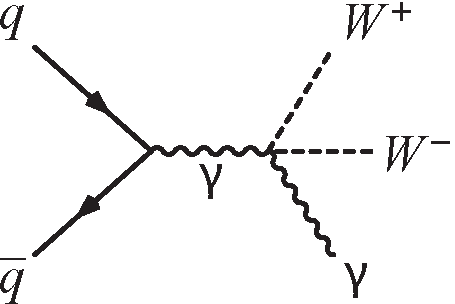
\includegraphics[width=0.3\textwidth]{figures/ss-inclboson-triboson-wvg-diagram1.pdf}
    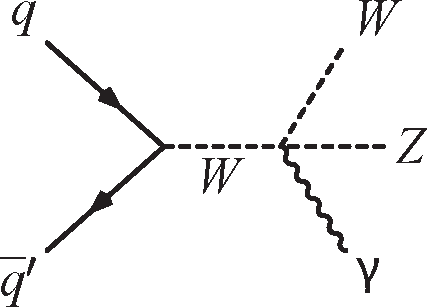
\includegraphics[width=0.3\textwidth]{figures/ss-inclboson-triboson-wvg-diagram2.pdf}
    \caption{Quartic gauge boson interaction Feynman diagrams for $WW\gamma$ and $WZ\gamma$ production~\cite{Chatrchyan:2014bza}.}
    \label{fig:ss-inclboson-triboson-wvg-diagrams}
\end{figure}


The photon $\ET$ of selected events is shown in
Fig.~\ref{fig:ss-inclboson-triboson-wvg-cms8tev}.  The leading
background is from $W\gamma$+jets production and is estimated from
extrapolation of the $m_{jj}$ sideband data into the signal region.
Multi-jet background is extrapolated from a control sample with low
$\MET$, and the other backgrounds such as top quarks are estimated
from simulation.  322 events are observed where $342\pm 16$ were
expected, of which 13 were expected to come from $WV\gamma$
production.  An upper limit at 95\% confidence level is obtained of
311 fb for the inclusive cross section, which is 3.4 times larger than
the standard model prediction of \texttt{aMC@NLO} ($91.6 \pm 21.7$ fb).

\begin{figure}[p]
    \centering
    \includegraphics[width=0.45\textwidth]{figures/ss-inclboson-triboson-wvg-ele-cms8tev.pdf}
    \includegraphics[width=0.45\textwidth]{figures/ss-inclboson-triboson-wvg-mu-cms8tev.pdf}
    \caption{Photon $\et$ distribution of $WV\gamma$ candidates selected by CMS~\cite{Chatrchyan:2014bza}.}
    \label{fig:ss-inclboson-triboson-wvg-cms8tev}
\end{figure}

The binned photon $\ET$ distribution in
Fig.~\ref{fig:ss-inclboson-triboson-wvg-cms8tev} is used to extract
limits on dimension 6 EFT couplings $a^W_0/\Lambda^2$ and
$a^W_C/\Lambda^2$, which affect $WW\gamma\gamma$ interactions, and
$\kappa^W_0/\Lambda^2$ and $\kappa^W_C/\Lambda^2$, which affect
$WWZ\gamma$ interactions.  The magnitude of the limits are in the
range of $12\ \textrm{TeV}^{-2}$ to $34\ \textrm{TeV}^{-2}$.  Limits
on the dimension 8 EFT couplings $f_{T,0}/\Lambda^4$,
$f_{M,0}/\Lambda^4$, $f_{M,1}/\Lambda^4$, $f_{M,2}/\Lambda^4$, and
$f_{M,3}/\Lambda^4$ are also obtained, in the range of
$25\ \textrm{TeV}^{-4}$ for $f_{T,0}/\Lambda^4$ and
$40-131\ \textrm{TeV}^{-4}$ for $f_{M,i}/\Lambda^4$.  


\section{Exclusive boson production}
\label{s-exclboson}
\subsection{Exclusive single boson production, vector-boson fusion}
\begin{figure}[p]
    \centering
    \includegraphics[height=0.3\textheight]{figures/ss-exclboson-z2j-atlas8tev}
    \caption{}
    \label{fig:ss-exclboson-z2j-atlas8tev}
\end{figure}
ATLAS VBF Z 7 \TeV~\cite{Aad:2014dta}

CMS VBF Z 7 \TeV~\cite{Chatrchyan:2013jya}

CMS VBF Z 8 \TeV~\cite{Khachatryan:2014dea}


\subsection{Exclusive di-boson production, vector-boson scattering}
%\begin{figure}[p]
%    \centering
%    \includegraphics[height=0.3\textheight]{figures/ss-exclboson-ww-cms7tev}
%    \caption{}
%    \label{fig:ss-exclboson-ww-cms7tev}
%\end{figure}
%CMS WWexcl 7 \TeV~\cite{Chatrchyan:2013foa}



\begin{figure}[htb]
\centering
%\includegraphics[width=.48\textwidth]{Figures/2016_01_29_UpdatedPlots/ee_pt.pdf}
\includegraphics[width=.48\textwidth]{figures/ss-exclboson-ww-cms8tev-1.pdf}
%\includegraphics[width=.48\textwidth]{Figures/2016_01_29_UpdatedPlots/ee_tracks_
%pt30.pdf}
\includegraphics[width=.48\textwidth]{figures/ss-exclboson-ww-cms8tev-2.pdf}
\caption{Evidence for exclusive diboson production via $pp \to p^{(*)}W^+ W^- p^{(*)} \to p^{(*)}\mu^{\pm}e^{\mp}p^{(*)}$.
Distributions of muon-electron transverse momentum for events with zero
 associated tracks (left), and extra-tracks multiplicity for events with $\pt(\mu^{\pm}e^{\mp}) > 30$\GeV (right).
 The data are shown by the points with error bars; the histograms indicate the expected SM signal and backgrounds.
\label{fig:ss-exclboson-ww-cms8tev}}
\end{figure}


\begin{figure*}[htb] {
\centering
\includegraphics[width=0.315\textwidth]{figures/ss-exclboson-ww-diagram1.pdf}
\includegraphics[width=0.35\textwidth]{figures/ss-exclboson-ww-diagram2.pdf}
\includegraphics[width=0.315\textwidth]{figures/ss-exclboson-ww-diagram3.pdf}
\caption{
Representative Feynman diagrams for same-sign $WW$ production in association
with two jets from purely electroweak contributions:
(left) vector boson fusion,
(middle) bremsstrahlung-like,
and (right) multiperipheral production.
\label{fig:ss-exclboson-ww-sigdiagram}}

}
\end{figure*}


\begin{figure}[p]
    \centering
    \includegraphics[width=0.45\textwidth]{figures/ss-exclboson-ww-ss-atlas8tev.pdf}
    \includegraphics[width=0.45\textwidth]{figures/ss-exclboson-ww-ss-cms8tev.pdf}
    \caption{
    Left:  a signal region by ATLAS.
    Right:  }
    \label{fig:ss-exclboson-ww-ss}
\end{figure}
ATLAS SSWW 8 \TeV~\cite{Aad:2014zda}
CMS SSWW 8 \TeV~\cite{Khachatryan:2014sta}


\section{Electro-weak precision tests}

\label{s-ewk-prec-tests}
\subsection{$Z$ $A_{FB}$ and $\sin^2\theta^{eff}_{W}$}
%ATLAS weak mixing angle~\cite{Aad:2015uau}

%CMS weak mixing angle~\cite{Chatrchyan:2011ya}

%CMS Drell--Yan AFB 7 \TeV~\cite{Chatrchyan:2012dc}

%CMS Drell--Yan AFB 8 \TeV (CMS-PAS-SMP-14-004, to be published)
\begin{figure}[p]
    \centering
    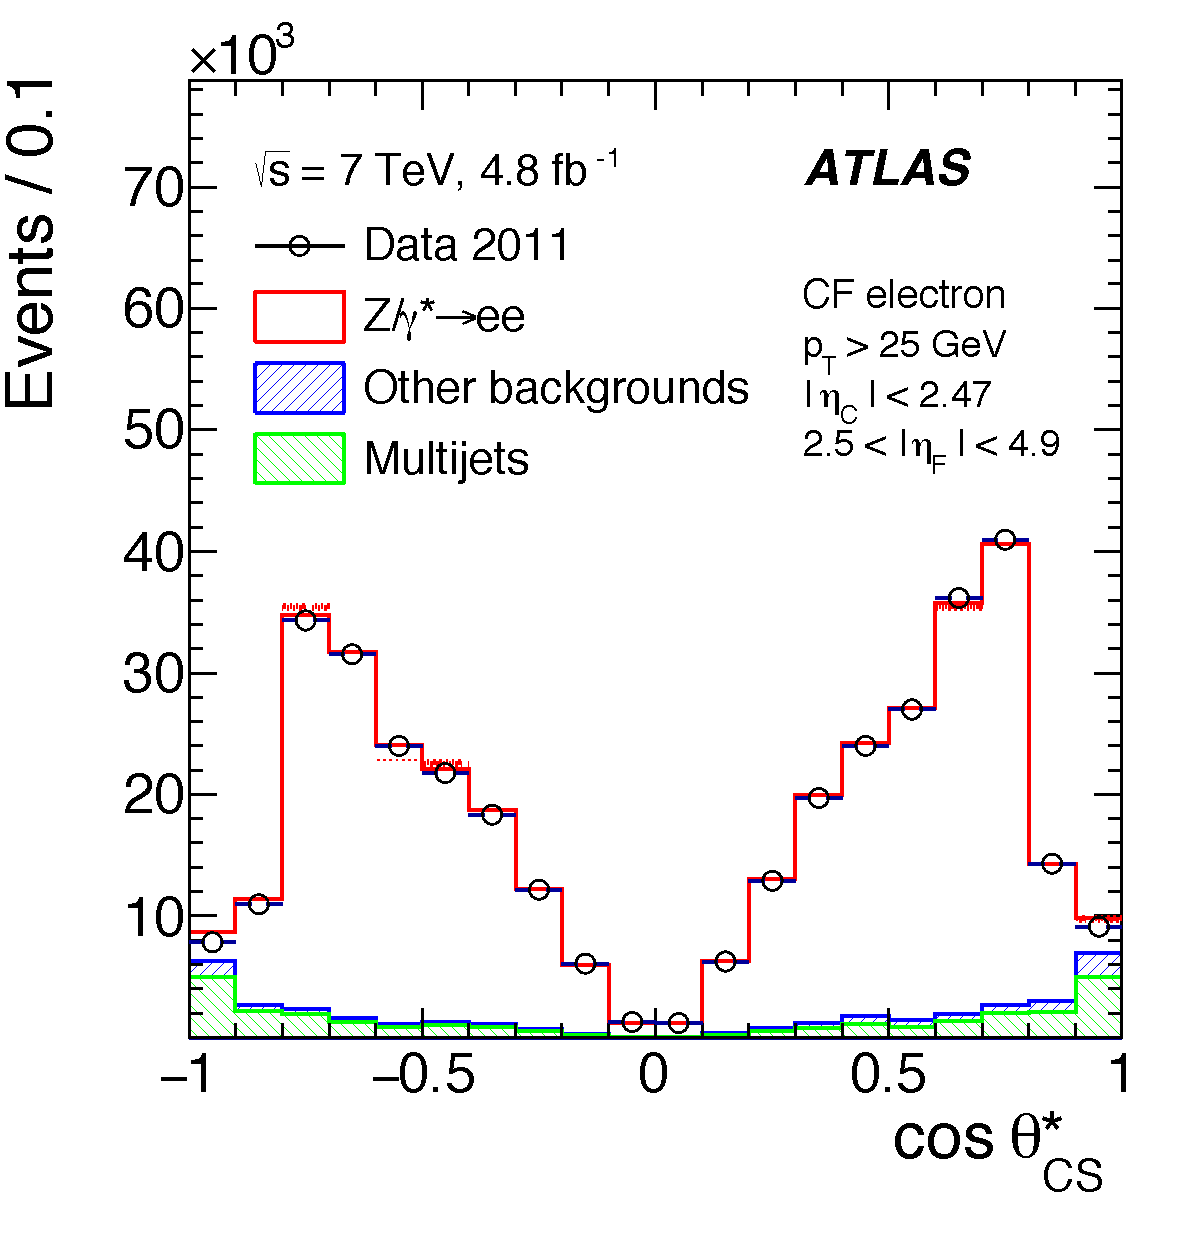
\includegraphics[width=0.45\textwidth]{figures/ss-precision-afb-atlas-cf-ct.pdf}
    \includegraphics[width=0.45\textwidth]{figures/ss-precision-afb-atlas-cf-afb.pdf}
    \caption{
    Left:  a signal region by ATLAS.
    Right:  }
    \label{fig:ss-precision-afb-atlas-cf}
\end{figure}
\begin{figure}[p]
    \centering
    \includegraphics[height=0.3\textheight]{figures/ss-precision-afb-atlas-sin2thetaw.pdf}
    \caption{}
    \label{fig:ss-precision-afb-atlas-sin2thetaw}
\end{figure}


\subsection{$W$ boson mass}

As discussed in the previous subsection, high-precision electroweak
observables are interrelated, and can be combined to predict any
other; deviations from expectations would be evidence for anomalous
interactions contributing to the loop corrections which influence
them.  The mass of the $W$ boson is a signifcant constraint on the
others; historically it has served as a predctive guide in the search for
both the top quark and the Higgs boson.  Now that both of those have been
measured precisely, the situation has reversed, and they can be used
to predict a value for $M_W$ of $80.358 \pm 0.008$
GeV~\cite{Baak:2014ora}, in comparison to the direct experimental
measurement $80.385 \pm 0.015$ GeV~\cite{Aaltonen:2013iut}, motivating
an improvement in precision by at least a factor of two.

The LHC experiments have not yet produced a measurement of the $W$
boson mass, but it is a stated goal of ATLAS, CMS, and LHCb to achieve
precision competitive with the world average.  The statistical
uncertainty of Run 1 data samples should be adequate to achieve this;
CMS analyses of Run 1 data selected over 120 million $W$ candidates
with good signal purity in the muon channel
alone~\cite{Chatrchyan:2013mza,Khachatryan:2016pev}, whereas the best
single measurements from the
Tevatron~\cite{Aaltonen:2012bp,Abazov:2012bv} currently use roughly 1
million events each.  Among others, the LHC experiments face
additional challenges, however.

The $W$ mass is typically estimated from the lepton $\pt$ or
lepton-$\MET$ transverse mass distributions.  This incomplete
reconstruction introduces modelling uncertainties from PDFs. In
proton-proton collisions at 7 TeV and higher, $W$ production has both
valence quark/sea anti-quark and sea quark/sea anti-quarkcomponents,
whereas proton--anti-proton collisions are predominantly valence
quark/valence anti-quark.  The latter are much better constrained
experimentally than the former, and so signifcant progress must be
made on sea quark PDFs to reduce associated $W$ mass uncertainties to
competitive levels.

Another important modelling uncertainty is the $W$ boson transverse
momentum.  This modelling has perturbative, non-perturbative, and PDF
uncertainties. Previous measurements have attempted to constrain these
by precisely measuring the $Z$ boson $\pt$, which constrain underlying
model parameters for both the $W$ and $Z$ spectra, and then translate
those to the $W$ $\pt$ spectrum. 

A related issue is the measurement of $\MET$ in the presence of
pileup.  If transverse mass is to be a competitive observable for
estimating $M_W$ throughout the Run 1 data sample, the resolution must
be competitive in pileup conditions of up to 25 interactions per bunch
crossing.  


%CDF W mass PRD~\cite{Aaltonen:2013vwa}
%CDF W mass PRL~\cite{Aaltonen:2012bp}

%D0 W asymmetry electron~\cite{Abazov:2013dsa}
%D0 W asymmetry muon~\cite{Abazov:2013rja}
%D0 W mass PRD~\cite{D0:2013jba}
%D0 W mass PRL~\cite{Abazov:2012bv}

%CDF+D0 W mass combination~\cite{Aaltonen:2013iut}

%Snowmass electroweak~\cite{Baak:2013fwa}

%Wmass PDF~\cite{Bozzi:2011ww}


\section{Summary}
%Summary & Outlook
The ATLAS and CMS experiments at the LHC have published a first set of electroweak measurements with the 
Run 1 data at a collision energy of $7\TeV$ and $8\TeV$,
%, and some first measurements with run-2 data at $\rts=13\TeV$. 
probing the electroweak sector at the hitherto highest available scales.
%DY
We started with the discussion of precision measurements of Drell-Yan production, a well understood electroweak
process that in turn is used to validate theoretical calculations with higher order corrections in
$\alpha_s$ and the PDF's of the proton. The total and differential cross section measurements help to 
reduce the theoretical cross section uncertainties of multi-boson processes, which are generally of the same order as the current
experimental uncertainties.  
%diboson
We reviewed the set of results available so far on inclusive di-boson production at the LHC. All inclusive di-boson final states
($\WW,\WZ,\ZZ,\Wg,\Zg$) have been observed and cross section measurements are available for collision energies of 7 TeV and 8 TeV. 
The complete set of measurements from both ATLAS and CMS including leptonic and semi-leptonic decay channels
is expected to be published towards the end of 2016.
%WWW+VBS
A highlight of the electroweak physics program at the LHC is the observation of electroweak production channels 
that became accessible for the first time, namely processes with 
three vector bosons in the final state, and vector boson scattering processes that are 
characterized by two forward jets and two vector bosons in the final state.

%aGC limits
For most total and fiducial cross section measurements with the full Run 1 dataset the systematic uncertainties 
already limit the precision. The exceptions are processes with cross sections below a few fb, e.g. tri-boson production. 
To probe the validity of the standard model at high partonic center-of-mass energy the limits
set in the framework of anomalous gauge couplings are surpassing legacy measurements at LEP and the Tevatron,
and are expected to further improve with increased $\rts$ and integrated luminosity. 

%legacy run-1 results
The set of Run 1 results, once completed, will present a unique legacy of electroweak precision results at 
$\rts$ values of 7 and 8 TeV.
%outlook
Run 2 analysis will extend the energy range to $\rts=13\TeV$ 
and provide even more sensitivity to anomalous gauge couplings. Potentially, 
the combination of ATLAS and CMS results will allow for more stringent constraints. In addition, the combination
with Higgs measurements in the framework of EFT with shared anomalous coupling operators is being 
actively pursued and will allow a further reduction of the allowed parameter space. 
Precision measurements or first observations of more tri-boson production and VBS processes will also become possible with the full 
Run 2 data set. 


 


\ack
Acknowledgments go here.

\bibliographystyle{iopart-num}
\bibliography{ewkrun1_master}

\end{document}
